\section{Results}
\label{sec:results}

\subsection{Pilot cohort: motivating result}

In the pilot cohort (GSE81089, NSCLC bulk RNA-seq, $n=218$), real data's $\maxHone$ significantly exceeds both null models in raw feature space ($z=26.1$ vs.\ Gaussian, $z=14.9$ vs.\ pipeline-symmetric permutation) and in PCA(50)-reduced space ($z=5.19$ vs.\ Gaussian, $z=5.23$ vs.\ permutation), supporting $H_0^{\text{stat}}$ in this cohort. However, the PCA-driven increase in $\maxHone$ observed in the real data ($\Delta = 0.78$) is \emph{smaller} than the PCA-driven increase observed in either null model applied to the same pipeline (Gaussian null $\Delta = 2.00 \pm 0.34$; pipeline-symmetric null $\Delta = 1.50 \pm 0.39$), i.e.\ PCA inflates persistence in unstructured noise \emph{more} than it does in the real NSCLC data. This is the pilot's motivating finding for $H_1^{\text{stat}}$ and is shown in \Cref{fig:fig1}: naive reporting of the PCA-space $H_1$ feature alone, without this comparison, would have overstated the topological claim.

\begin{figure}[htbp]
\centering
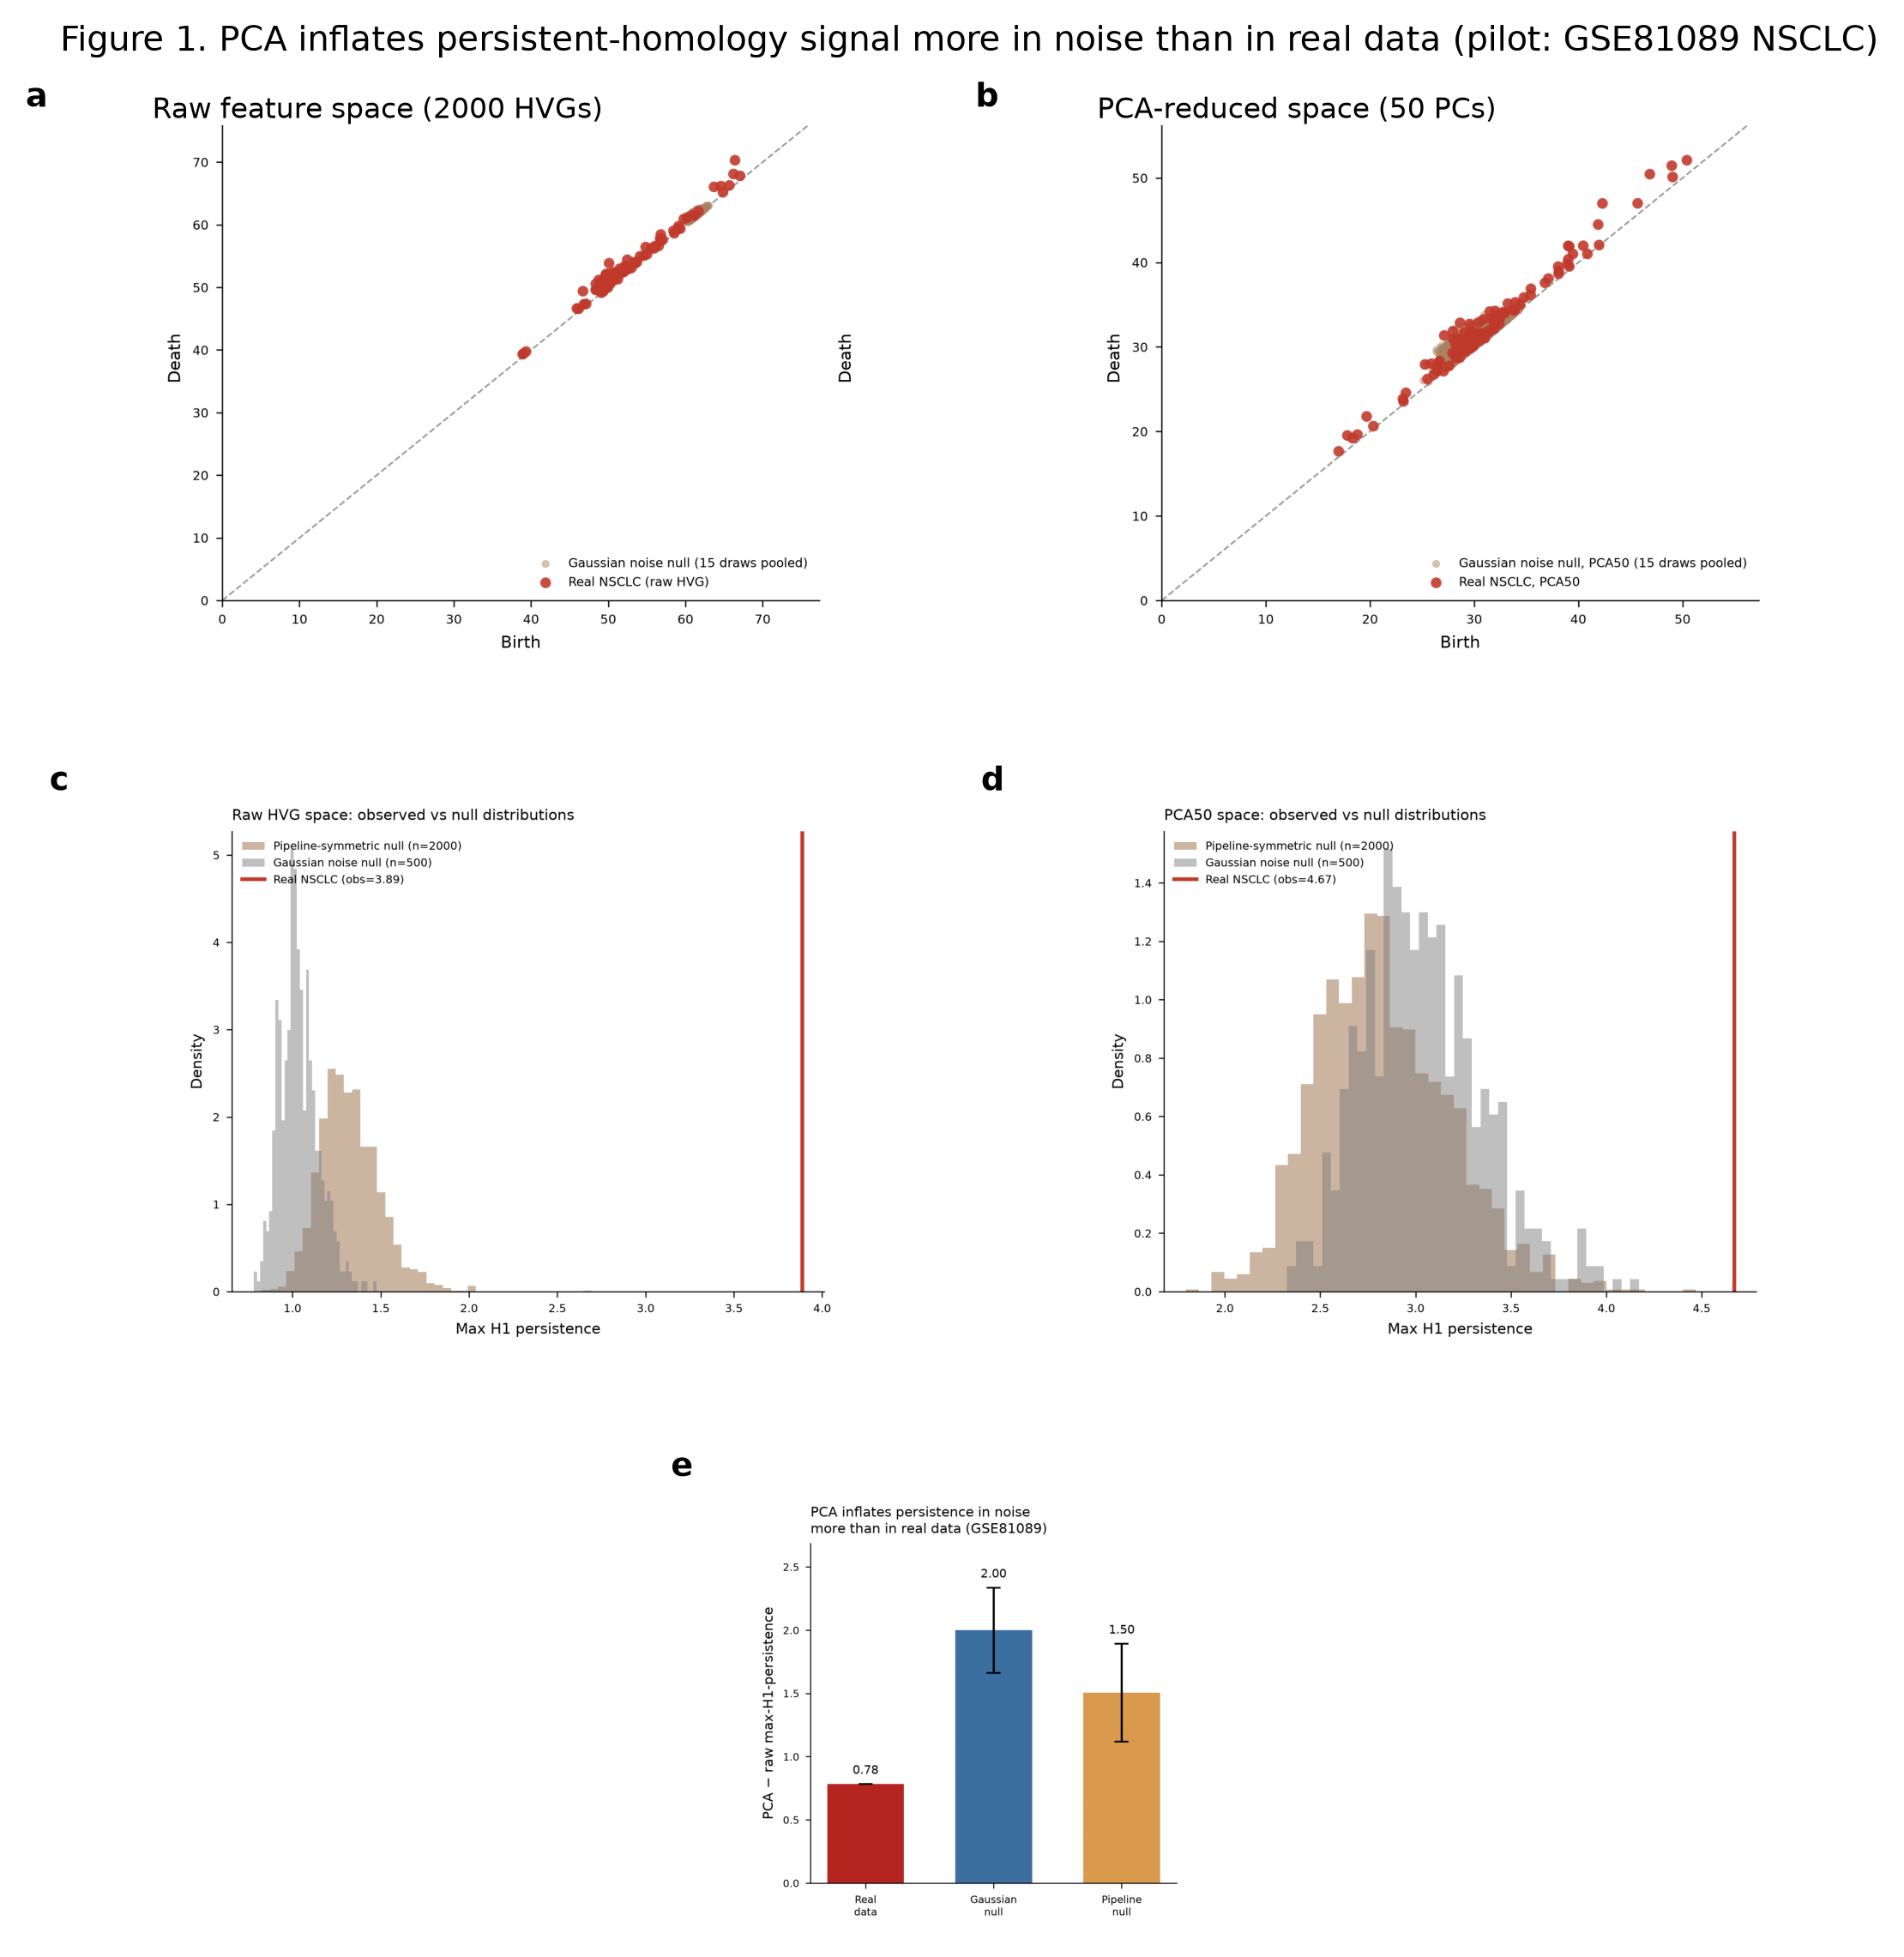
\includegraphics[width=0.95\textwidth]{figures/fig1_pilot_motivation.png}
\caption{\textbf{PCA amplifies persistent-homology signal in noise as much as in real data (pilot cohort, GSE81089 NSCLC).} (a--b) $H_1$ persistence diagrams, real data (red) vs.\ pooled Gaussian-noise null (tan), in raw feature space (a) and PCA(50)-reduced space (b); real points shift further above the diagonal in PCA space, but so does the null. (c--d) Observed $\maxHone$ (vertical red line) against the pipeline-symmetric permutation null (tan) and Gaussian null (grey) distributions, in raw (c) and PCA (d) space; real data exceeds both nulls by a wide margin in both spaces ($H_0^{\text{stat}}$ supported). (e) The PCA-driven $\Delta$ in $\maxHone$ is smaller in real data (0.78) than in either null model (Gaussian: 2.00; pipeline-symmetric: 1.50), showing PCA's persistence-inflating effect on this cohort's noise floor is larger than its effect on the real signal.}
\label{fig:fig1}
\end{figure}

\subsection{Cross-dataset replication}

The three confirmatory cohorts (GSE146889, CPTAC-CCRCC, TCGA-LUAD) contribute 16 pre-registered, BH-FDR-corrected tests of $H_0^{\text{stat}}$ (\Cref{tab:h0-crossdataset}). 14 of 16 (87.5\%) pass at BH-adjusted $\alpha=0.05$ and the pre-registered $z>3.0$ threshold. The two failures are both in the same feature space: TCGA-LUAD's methylation data, after PCA(35, spectral metric), shows real $\maxHone$ collapsing to zero, so neither the Gaussian ($z=-0.20$) nor permutation ($z=-0.79$) comparison can register a signal --- this is a failure of the real signal to survive PCA in that specific modality, not a failure of the null models.

\begin{table}[htbp]
\centering
\small
\caption{$H_0^{\text{stat}}$ cross-dataset replication: $z$-scores vs.\ matched nulls, raw and PCA-reduced space. All effect sizes clear $z>3.0$ except TCGA-LUAD methylation PCA (both nulls).}
\label{tab:h0-crossdataset}
\begin{tabular}{@{}llrrl@{}}
\toprule
Dataset & Layer / space & $z$ (Gaussian) & $z$ (permutation) & BH-corrected pass \\
\midrule
GSE81089 (pilot)\footnotemark[1] & RNA-seq, raw & 26.06 & 14.92 & --- \\
GSE81089 (pilot)\footnotemark[1] & RNA-seq, PCA50 & 5.19 & 5.23 & --- \\
GSE146889 & RNA-seq, raw & 44.87 & 39.59 & Yes \\
GSE146889 & RNA-seq, PCA50 & 12.02 & 11.37 & Yes \\
CPTAC-CCRCC & Proteomics, raw & 23.18 & 21.39 & Yes \\
CPTAC-CCRCC & Proteomics, PCA50 & 4.40 & 4.64 & Yes \\
TCGA-LUAD & RNA-seq, raw & 58.67 & 47.53 & Yes \\
TCGA-LUAD & RNA-seq, PCA50 & 9.19 & 8.34 & Yes \\
TCGA-LUAD & Methylation, raw & 19.34 & 26.69 & Yes \\
TCGA-LUAD & Methylation, PCA35 (spectral) & $-0.20$ & $-0.79$ & \textbf{No} \\
\bottomrule
\end{tabular}
\vspace{2pt}
\footnotesize{\footnotemark[1]Pilot cohort shown for reference; not part of the pre-registered confirmatory BH-FDR family.}
\end{table}

Table~\ref{tab:h1-crossdataset} reports the $H_1^{\text{stat}}$ (PCA-attribution) comparison in every cohort and layer: the real PCA-driven $\Delta$ in $\maxHone$ against the range spanned by the two null models' own PCA-driven $\Delta$. In GSE81089, GSE146889, and CPTAC-CCRCC, the real $\Delta$ is positive but smaller than both null $\Delta$s --- the pre-registered, literal form of $H_1^{\text{stat}}$ holds in each. TCGA-LUAD RNA-seq shows a stronger form of the same conclusion: the real $\Delta$ is \emph{negative} ($-0.89$), i.e.\ PCA in this cohort's RNA-seq layer actually \emph{reduces} $\maxHone$ relative to raw space, while both nulls show a positive inflation of $+2.35$ to $+2.51$ --- an even larger gap disfavoring the naive interpretation. TCGA-LUAD's methylation layer is a distinct case: the real $\Delta$ is strongly negative ($-4.09$), driven by the real signal's near-total collapse under PCA(35, spectral) noted above, while the null $\Delta$s are mildly negative ($-0.90$ to $-0.79$); this is consistent with $H_1^{\text{stat}}$ but for a different underlying reason (loss of real signal rather than a comparable but smaller inflation).

\begin{table}[htbp]
\centering
\small
\caption{$H_1^{\text{stat}}$ cross-dataset replication: real PCA-driven $\Delta$(max-$H_1$) vs.\ range spanned by null models' own $\Delta$.}
\label{tab:h1-crossdataset}
\begin{tabular}{@{}lrrl@{}}
\toprule
Dataset / layer & Real $\Delta$ & Null $\Delta$ range & $H_1^{\text{stat}}$ verdict \\
\midrule
GSE81089 (pilot) & $+0.78$ & $[1.50, 2.00]$ & Supported \\
GSE146889 & $+1.36$ & $[2.08, 2.18]$ & Supported \\
CPTAC-CCRCC & $+0.85$ & $[2.01, 2.10]$ & Supported \\
TCGA-LUAD RNA-seq & $-0.89$ & $[2.35, 2.51]$ & Supported (stronger form) \\
TCGA-LUAD Methylation & $-4.09$ & $[-0.90, -0.79]$ & Supported (distinct mechanism) \\
\bottomrule
\end{tabular}
\end{table}

\Cref{fig:fig2} summarizes both tables graphically alongside the confound cross-check (\Cref{sec:results-confound-crossdataset}).

\begin{figure}[htbp]
\centering
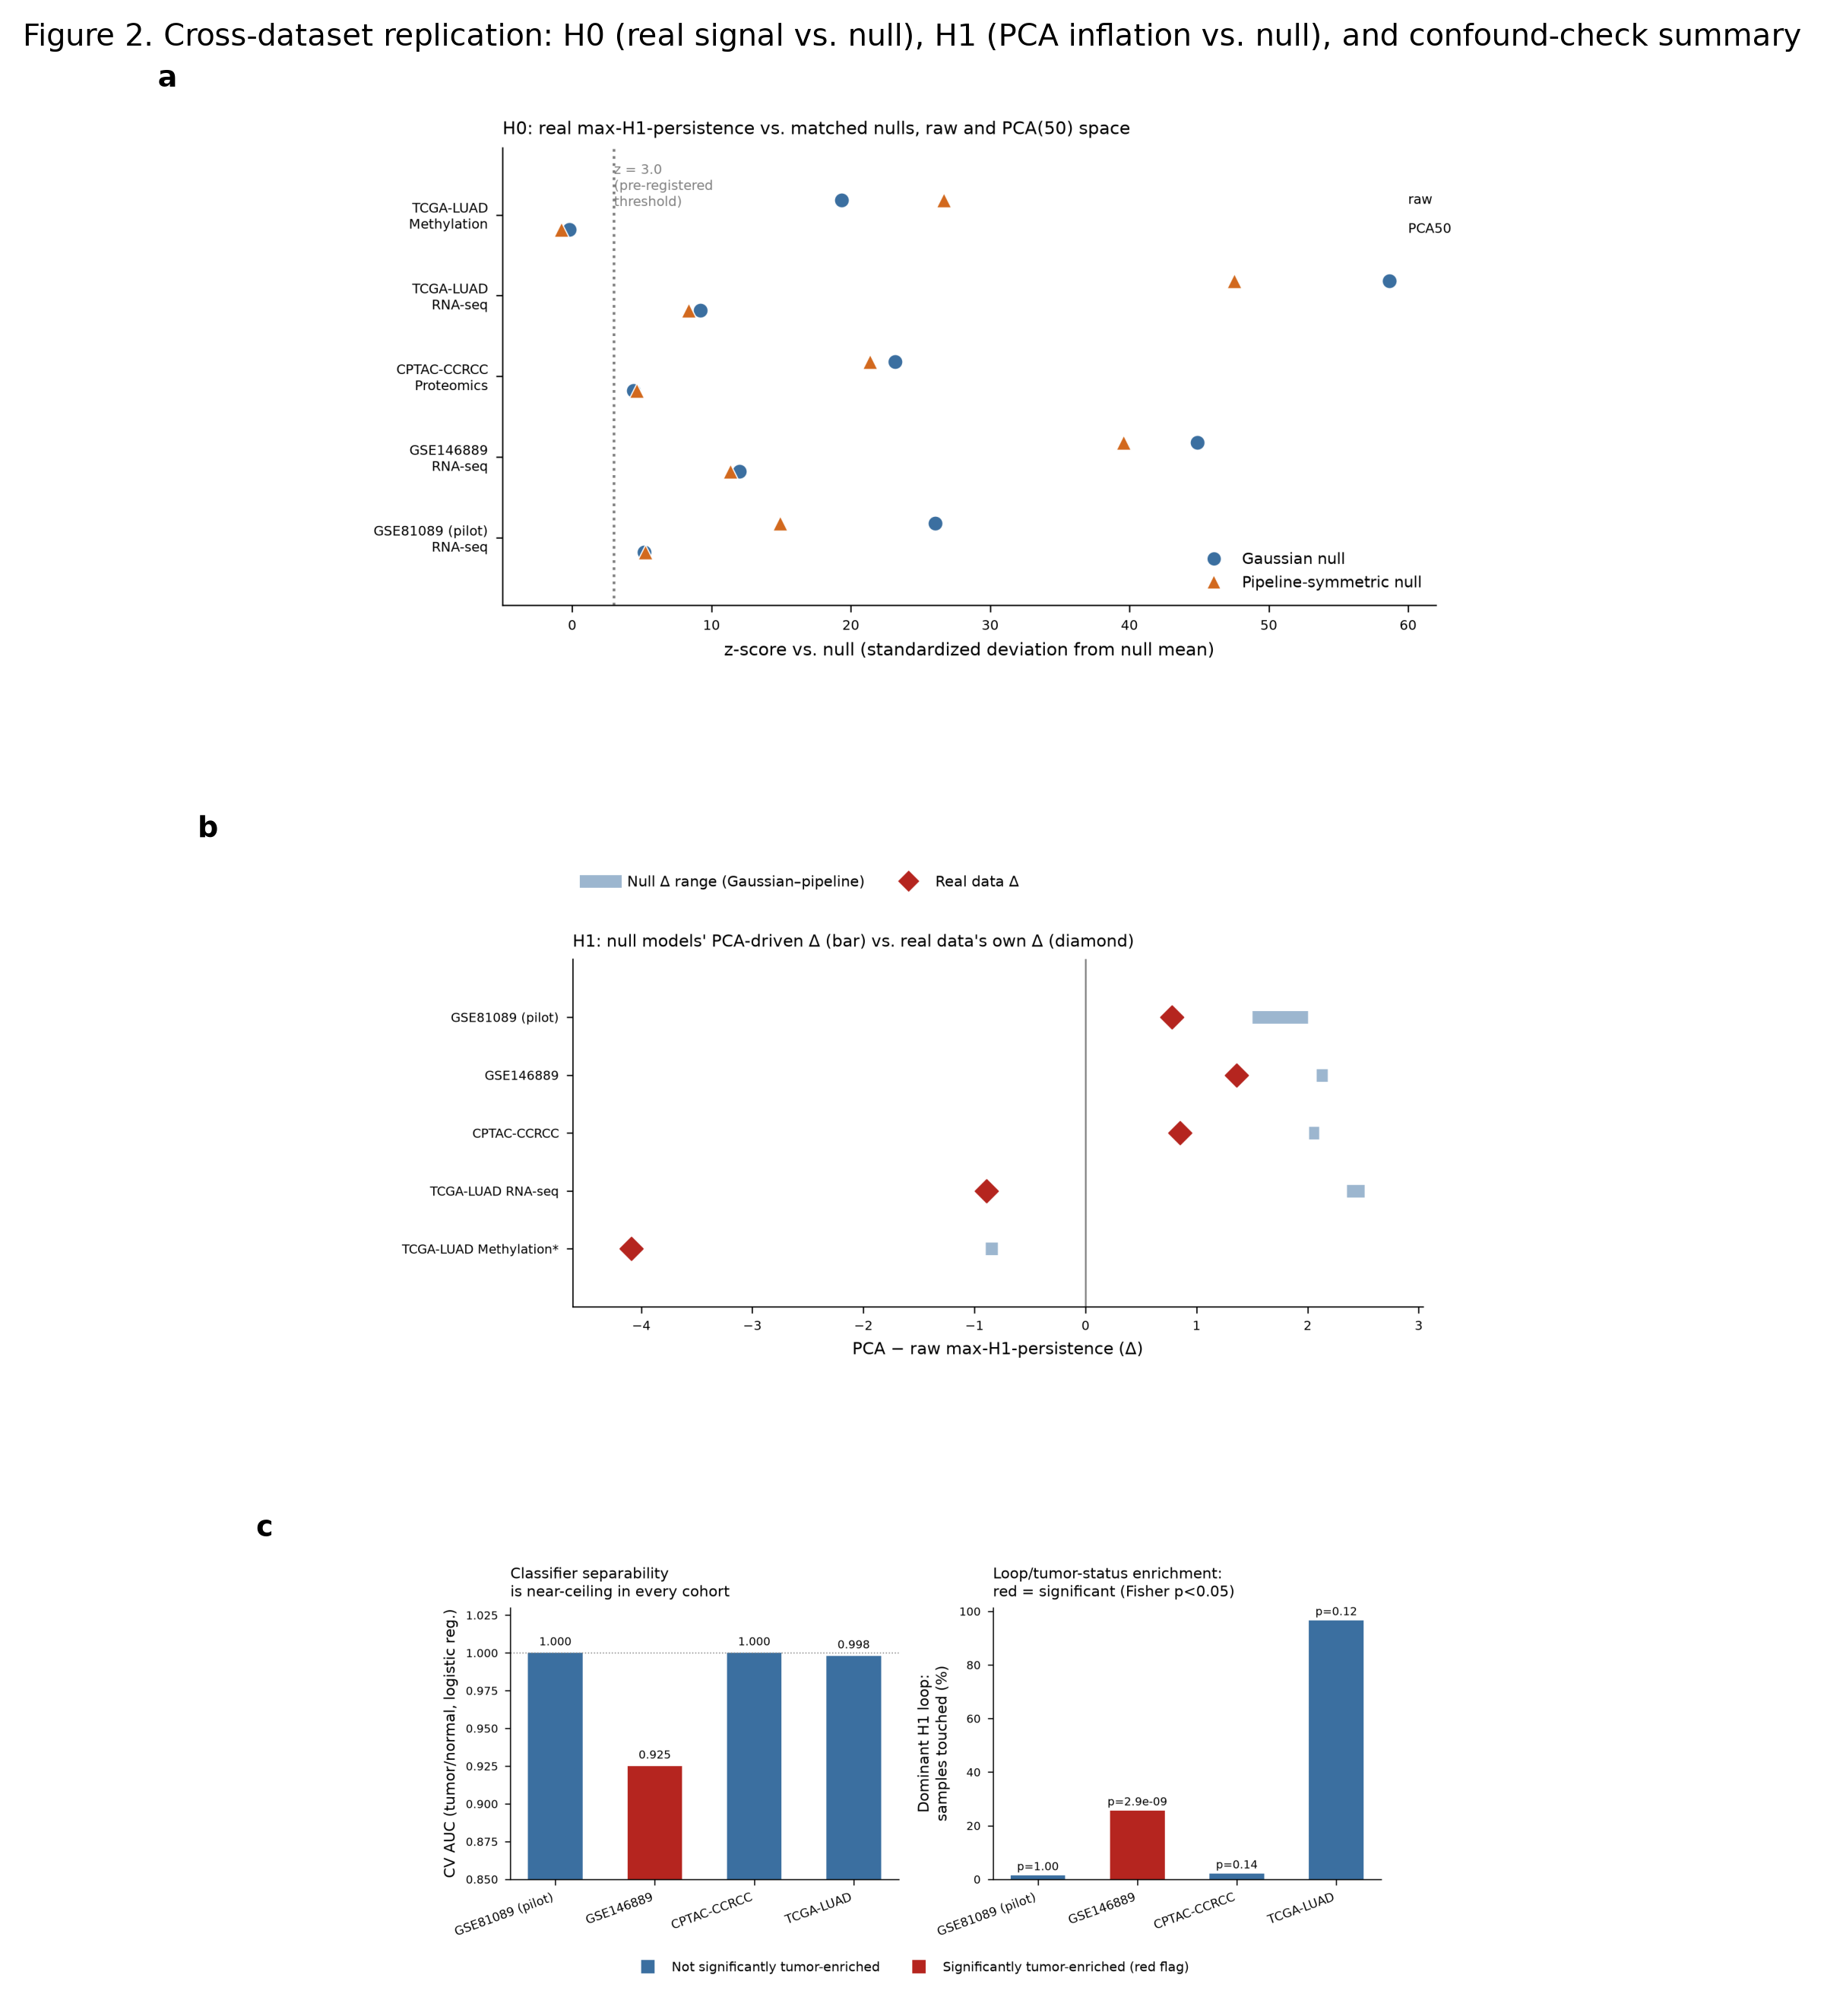
\includegraphics[width=0.92\textwidth]{figures/fig2_cross_dataset_replication.png}
\caption{\textbf{Cross-dataset replication summary.} (a) $H_0^{\text{stat}}$: $z$-scores of real $\maxHone$ vs.\ Gaussian (circle) and pipeline-symmetric (triangle) nulls, raw and PCA(50) space, across all five cohort/layer combinations; dotted line marks the pre-registered $z=3.0$ threshold. All comparisons clear threshold except TCGA-LUAD methylation PCA space. (b) $H_1^{\text{stat}}$: real PCA-driven $\Delta$ in $\maxHone$ (diamond) against the range spanned by the two null models' own PCA-driven $\Delta$ (bar); real $\Delta$ falls at or below the null range in every cohort. (c) Confound cross-check: cross-validated classifier AUC for tumor/normal status (left) and the fraction of samples touched by the dominant $H_1$ loop, colored by whether that loop is significantly enriched for tumor status (Fisher's exact test, right). GSE146889 is flagged red: its loop is significantly tumor-enriched, unlike the other three cohorts.}
\label{fig:fig2}
\end{figure}

\subsection{Confound cross-check across cohorts}
\label{sec:results-confound-crossdataset}

Independent of the full confound-\emph{attribution} audit (\Cref{sec:methods-confound}, applied to date only to the pilot cohort), each replication report includes a lighter cross-check: cross-validated tumor/normal classifier AUC, and whether the dominant $H_1$ loop's participating samples are significantly enriched for one class (Fisher's exact test). Classifier AUC is at or near ceiling in every cohort (GSE81089: 1.000; GSE146889: 0.925; CPTAC-CCRCC: 1.000; TCGA-LUAD: 0.918--0.998 across spaces) --- the tumor/normal distinction is linearly separable everywhere, which is precisely why the confound-attribution question in \Cref{sec:methods-confound} is worth asking at all. The dominant-loop enrichment check, however, differs sharply across cohorts: GSE81089's loop touches only 3/218 samples and is not significantly enriched (Fisher $p=1.0$); CPTAC-CCRCC's loop touches 3--4/194 samples, also not significant ($p>0.13$); TCGA-LUAD's loop touches 112/116 samples (essentially the whole cohort) and is not significantly enriched relative to overall tumor fraction ($p=0.12$). GSE146889 is the exception: its dominant loop touches 45/176 samples and \emph{is} significantly enriched for tumor status (odds ratio 12.5, Fisher $p=2.9\times10^{-9}$) --- a structurally different pattern from the pilot's clean, non-enriched loop, and the specific reason the pilot's confound-audit conclusion (\Cref{sec:results-confound}) cannot be assumed to generalize to GSE146889 without direct testing.

\subsection{Ablation / hyperparameter-sensitivity sweep}

The 18-configuration sweep on the pilot cohort (\Cref{fig:fig3}) shows $H_1^{\text{stat}}$ is directionally robust at the pre-registered operating point (HVG$=2000$, PC$=50$) and across most of the sampled grid (14/18 configurations, 78\%, support $H_1^{\text{stat}}$ against both nulls simultaneously; $H_0^{\text{stat}}$ holds in 16/18, 89\%), but fails in two distinct, identifiable regimes:

\begin{enumerate}
\item \textbf{Low PC count (PC=10), dominant failure mode.} At PC$=10$, across all three HVG settings tested at that PC count (500, 2000, 4000), the real PCA-driven $\Delta$ (1.36--5.65) exceeds \emph{both} null models' $\Delta$ --- the direction of the pre-registered $H_1^{\text{stat}}$ inequality reverses. Aggressive dimensionality reduction to very few components appears to let the real data's structure dominate the projection in a way the null pipeline does not reproduce at the same PC count.
\item \textbf{High gene-count / high PC-count (HVG=4000, PC=100), secondary failure mode.} At this corner, the real $\Delta$ (2.45) exceeds the pipeline-symmetric null's $\Delta$ (2.36) --- $H_1^{\text{stat}}$ fails specifically against the more conservative permutation null, despite highly significant $z$-scores against the null distributions overall (raw-space $z=20.4$ vs.\ pipeline, $z=28.2$ vs.\ Gaussian) --- while still passing against the Gaussian null ($\Delta=2.75$).
\end{enumerate}

Permutation count converged well before the pre-registered $n=2000$ (bootstrapped 95\% CI on the $z$-score stabilizes by $n\approx250$--$500$ for both raw- and PCA-space comparisons). Missing-value imputation rule is essentially inconsequential to the HVG selection at the pre-registered operating point: pairwise Jaccard overlap of the selected highly-variable gene sets across all four rules (zero, mean, median, drop) is $\geq0.97$, and all four rules agree on which samples participate in the dominant $H_1$ loop (Jaccard $=1.000$). The gene-count $\times$ PC-count interaction check (\Cref{fig:fig3}b) finds the observed joint effect exceeds the additive (leave-one-out-summed) prediction from each hyperparameter's marginal effect at all four grid corners, indicating a genuine superadditive interaction rather than two independent, additive nuisance effects.

\begin{figure}[htbp]
\centering
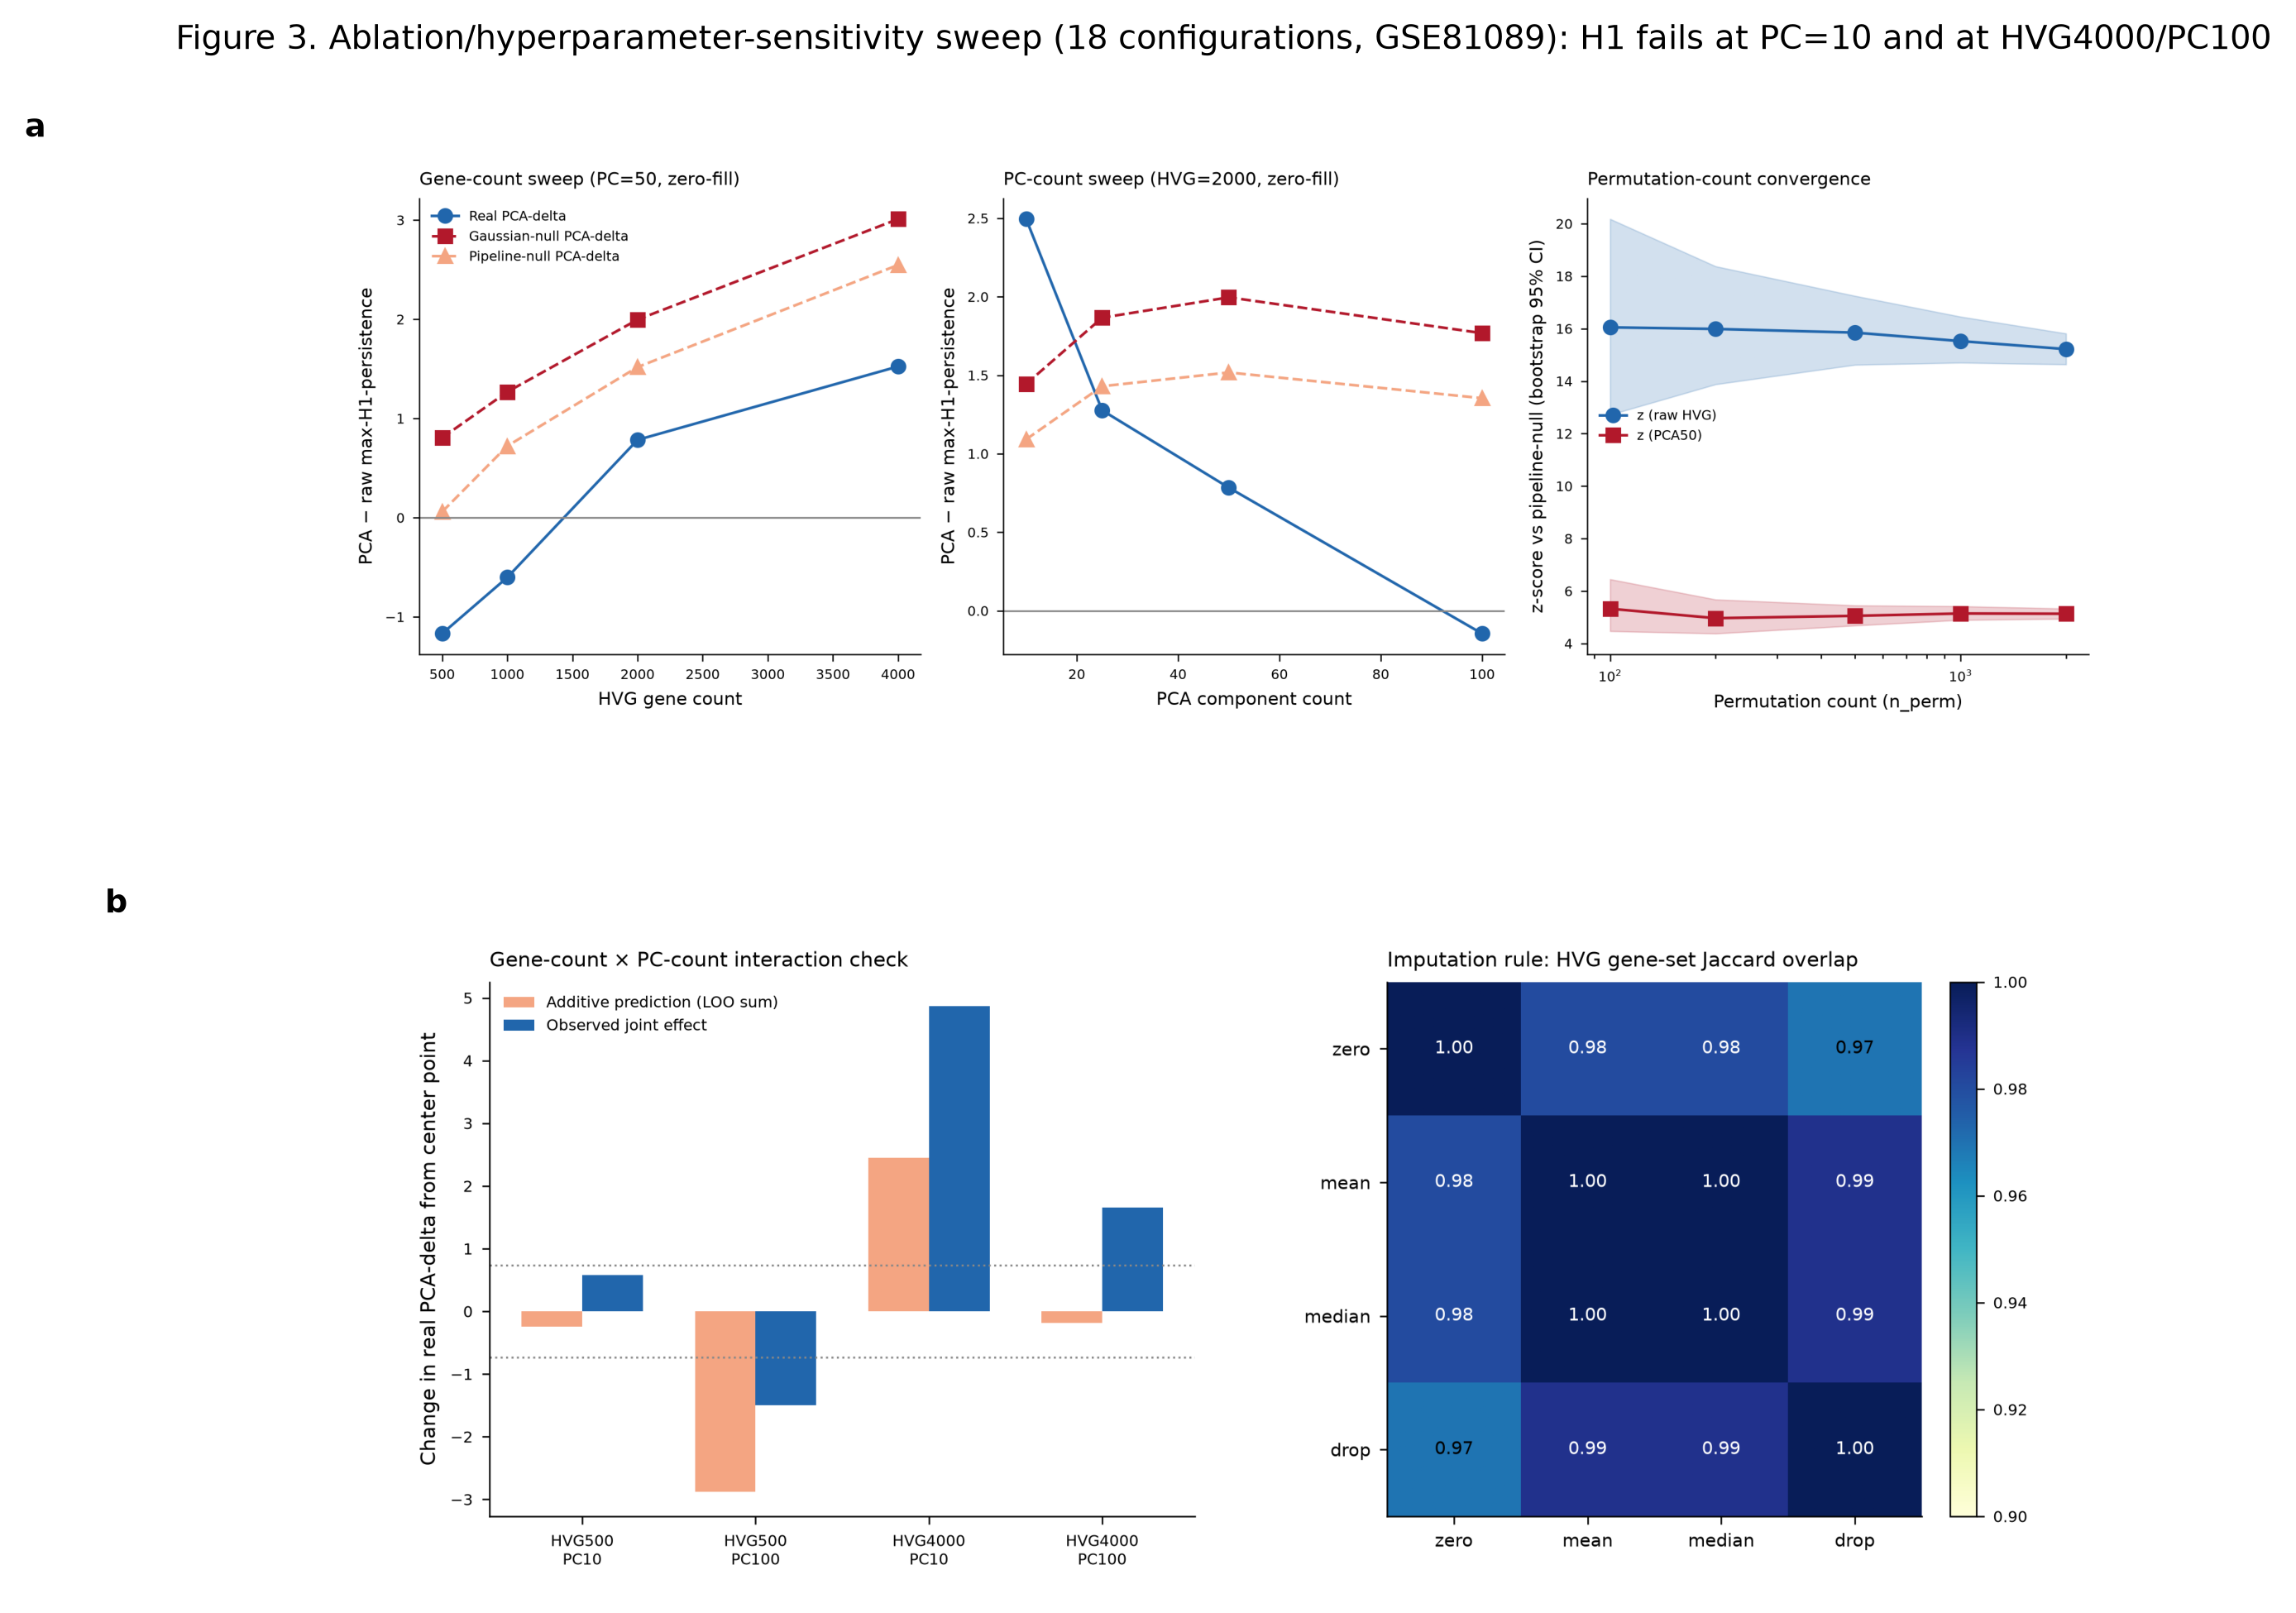
\includegraphics[width=0.95\textwidth]{figures/fig3_ablation_sensitivity.png}
\caption{\textbf{Ablation/hyperparameter-sensitivity sweep (18 configurations, pilot cohort GSE81089).} (a, left) Gene-count sweep at PC$=50$: real PCA-driven $\Delta$ (blue) crosses below zero at HVG$=500$ and again near HVG$=4000$ relative to the null $\Delta$s (red/orange), which remain positive throughout. (a, center) PC-count sweep at HVG$=2000$: real $\Delta$ exceeds both null $\Delta$s at PC$=10$, the dominant failure mode, then falls below both nulls from PC$=25$ onward. (a, right) Permutation-count convergence: $z$-scores vs.\ pipeline-symmetric null stabilize well before the pre-registered $n=2000$. (b, left) Gene-count $\times$ PC-count interaction check: observed joint effect (blue) vs.\ additive prediction (orange) at the four grid corners; all four corners show superadditive interaction. (b, right) Imputation-rule HVG gene-set Jaccard overlap: all pairwise overlaps $\geq0.97$.}
\label{fig:fig3}
\end{figure}

\subsection{Confound-attribution audit: pilot cohort (GSE81089)}
\label{sec:results-confound}

Having established that $H_1^{\text{stat}}$ (PCA-attribution) is robust at the pre-registered operating point in the pilot cohort, the confound-attribution audit (\Cref{sec:methods-confound}) asks a distinct question: is the residual topological signal that does survive both nulls at the pre-registered operating point attributable to the tumor/normal class-mean shift, or independent of it? \textbf{This audit has been completed, at the time of writing, only for the pilot cohort, GSE81089.} We report its result here scoped explicitly to this one cohort; whether it generalizes to the three replication cohorts is an open question (\Cref{fig:fig4}c).

In GSE81089, the tumor/normal class-mean-shift direction correlates strongly with PC1 ($r=0.865$) and a linear classifier recovers tumor/normal status from the top discriminant direction alone at $\mathrm{AUC}=0.9995$. Despite this, four independent lines of evidence indicate the $H_1$ topological signal is not a re-description of that class-mean shift, within this cohort:

\begin{enumerate}
\item \textbf{Within-class decomposition.} Restricting to the tumor-only subpopulation ($n=199/218$) reproduces the identical $\maxHone$ statistic (3.887) found in the full mixed population, with strong significance against both nulls ($z=23.0$ Gaussian, $z=14.5$ permutation). The normal-only subpopulation ($n=19$) shows no comparable signal ($\maxHone=0.405$).
\item \textbf{Within-stratum control.} Stratifying the tumor-only subpopulation into quartiles along the class-mean-shift direction, the signal survives in every quartile ($z=8.8$--$28.4$ against the matched Gaussian null), ruling out a signal concentrated only in samples closest to the normal population along that axis.
\item \textbf{Residualization control.} After projecting out the class-mean-shift direction, $\maxHone$ remains high (3.731, vs.\ 3.887 unresidualized) and significant against the Gaussian null ($z=31.1$); against the more conservative pipeline-permutation null the residualized signal is $z=2.97$ --- just under the pre-registered $z>3.0$ threshold, a partial rather than unambiguous pass. Critically, a classifier trained on the residualized data to recover tumor/normal status collapses from $\mathrm{AUC}=1.000$ (unresidualized) to $\mathrm{AUC}=0.094$ (a permutation test on this collapse gives $p=0.005$), confirming the confound direction was successfully removed.
\item \textbf{Block-bootstrap confidence interval.} A block-bootstrap 95\% CI on the residual signal-beyond-null quantity is $[1.37, 3.77]$, excluding zero.
\end{enumerate}

\begin{figure}[htbp]
\centering
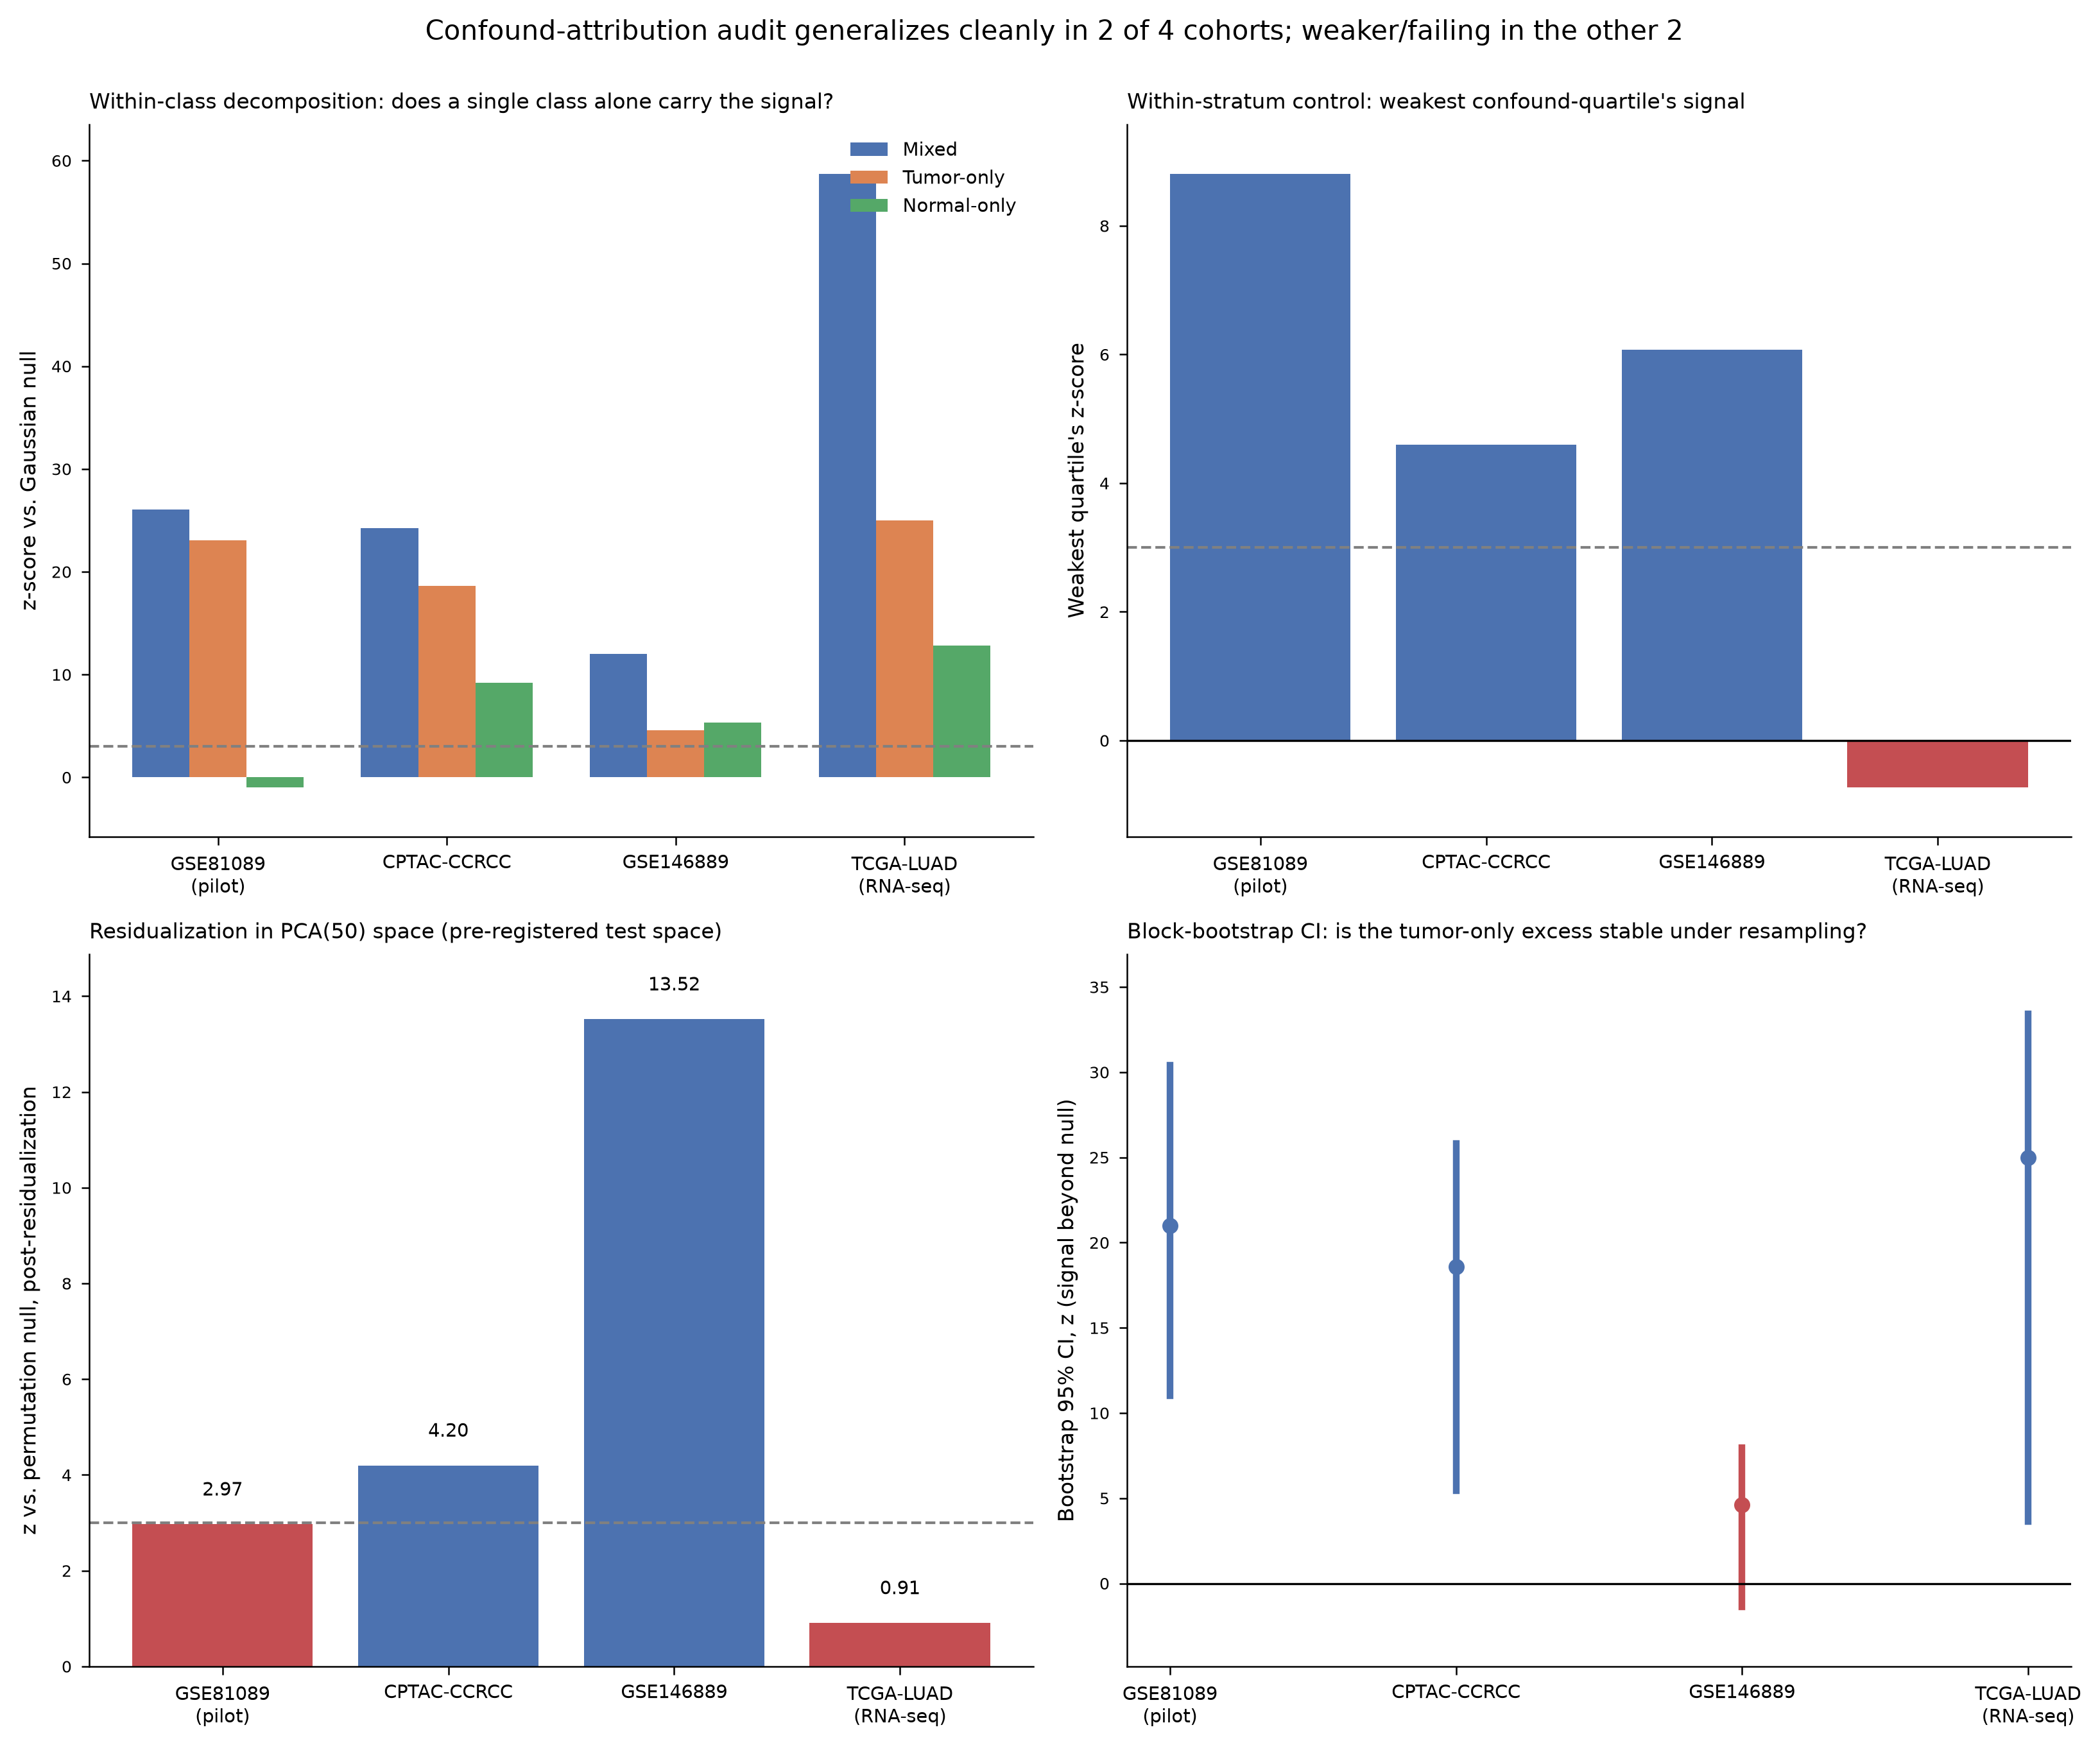
\includegraphics[width=0.92\textwidth]{figures/fig4_confound_audit.png}
\caption{\textbf{Confound-attribution audit across all four cohorts.} Dashed grey line marks the pre-registered $z=3.0$ threshold; bars/points below or crossing it are colored red. (a) Within-class decomposition: $z$-score (vs.\ Gaussian null) for the mixed population, tumor-only subset, and normal-only subset, in each cohort. GSE81089's underpowered normal-only arm ($n=19$) shows no excess; CPTAC-CCRCC's well-powered normal-only arm ($n=84$) does. (b) Within-stratum control: the \emph{weakest} confound-quartile's $z$-score in each cohort --- all clear threshold except TCGA-LUAD, where the least tumor-like quartile falls \emph{below} its own null mean. (c) Residualization in PCA(50) space --- the space this program's primary tests are run in --- against the more conservative permutation null: GSE81089 sits just at threshold ($z=2.97$), CPTAC-CCRCC and GSE146889 clear it, and TCGA-LUAD collapses to null-indistinguishable ($z=0.91$). (d) Block-bootstrap 95\% CI on the tumor-only signal-beyond-null ($z$-scale): GSE81089, CPTAC-CCRCC, and TCGA-LUAD exclude zero (TCGA-LUAD's lower bound is close to threshold); GSE146889 does not.}
\label{fig:fig4}
\end{figure}

\subsection{Confound-attribution audit: generalization to the three replication cohorts}
\label{sec:results-confound-generalization}

The same four-part audit protocol (\Cref{sec:methods-confound}) was subsequently applied, identically, to
GSE146889, CPTAC-CCRCC, and TCGA-LUAD (RNA-seq layer; the methylation layer was excluded because its
real PCA-space $\maxHone$ is already zero, so there is no signal to attribute). Each audit independently
re-verified its dataset's earlier pipeline numbers (real $\maxHone$, intrinsic dimension, classifier AUC)
to high precision before running any new test, confirming the reproduction was faithful. \Cref{tab:confound-crossdataset}
summarizes all four audits, including the pilot.

\begin{table}[htbp]
\centering
\small
\caption{Confound-attribution audit summary across all four cohorts. ``Within-class match'' asks whether a
single-class subset reproduces the mixed-population $\maxHone$ statistic; ``Within-stratum'' asks whether
every confound-quartile clears $z>3.0$; ``Residualization'' reports whether the aggregate signal survives
exact linear removal of the class-mean-shift direction (and, where relevant, in which feature space);
``Bootstrap CI'' reports whether the 95\% block-bootstrap CI on the signal-beyond-null excludes zero.}
\label{tab:confound-crossdataset}
\begin{tabular}{@{}p{2.6cm}p{2.6cm}p{2.3cm}p{3.6cm}p{2.6cm}p{2.6cm}@{}}
\toprule
Dataset & Within-class match & Within-stratum & Residualization & Bootstrap CI & Verdict \\
\midrule
GSE81089 (pilot) & Yes ($3.887=3.887$) & Yes ($z{=}8.8$--$28.4$) & Gaussian $z{=}31.1$; permutation $z{=}2.97$ (near-miss) & Yes, tumor-only $[1.37,3.77]$ & Genuine, tumor-scoped \\
CPTAC-CCRCC & Yes ($3.833=3.833$) & Yes ($z{=}4.6$--$11.3$) & Gaussian $z{=}36.5$; permutation $z{=}4.20$ (clears) & Yes, tumor-only $[0.83,3.96]$ & Genuine, extends to normal tissue \\
GSE146889 & \textbf{No} ($5.880$ vs.\ $7.564$, 78\%) & Yes ($z{=}6.1$--$23.6$)\footnotemark[1] & Clears aggregate stat ($z{=}14.4/13.5$) but dominant loop \emph{identity} changes & \textbf{No}, neither subset excludes 0 & Partially genuine, weaker \\
TCGA-LUAD (RNA-seq) & \textbf{No} ($4.596$ vs.\ $8.327$, 55\%) & \textbf{No} --- Q1 fails ($z{=}-0.73$) & Raw space survives but $=$ pre-existing normal-loop statistic; \textbf{PCA(50) space collapses} ($z{=}0.50/0.91$) & Marginal, lower bound $z{=}3.65$ & Mixed/weaker, fails in pre-registered space \\
\bottomrule
\end{tabular}
\vspace{2pt}
\footnotesize{\footnotemark[1]Quartiles here are not label-balanced (Q1 98\% normal, Q4 100\% tumor) because the classifier separates the classes cleanly along this exact projection.}
\end{table}

\textbf{Two of four cohorts (GSE81089, CPTAC-CCRCC) replicate the clean genuine-signal picture.}
CPTAC-CCRCC's audit reproduces every element of the pilot's decisive result: the tumor-only subset matches
the mixed-population statistic to six decimal places, every confound-quartile clears the significance bar,
and the residualized signal survives against \emph{both} nulls with more room than the pilot itself
($z=4.20$ vs.\ the pilot's near-miss $z=2.97$ against the permutation null). CPTAC-CCRCC additionally has a
well-powered normal-only arm ($n=84$, vs.\ the pilot's underpowered $n=19$) that also clears the null
threshold ($z=9.2$ Gaussian, $z=14.2$ permutation) --- a result the pilot could not establish either way,
extending rather than merely replicating the confound-independence finding to a second tissue compartment.

\textbf{The other two cohorts (GSE146889, TCGA-LUAD) do not.} GSE146889 passes the within-stratum control
and the residualization control at the level of the aggregate $\maxHone$ scalar, but fails the two controls
that gave the pilot its most decisive, assumption-light evidence: neither the tumor-only nor the
normal-only subset reproduces the mixed-population magnitude, and neither subset's bootstrap CI on the
signal-beyond-null excludes zero. Moreover, while the aggregate statistic survives residualization, the
\emph{specific dominant loop} does not --- a different set of 22 samples, at a near-baseline tumor/normal
composition (Fisher $p=0.65$), replaces the original 45-sample, tumor-enriched loop (Fisher $p=2.9\times10^{-9}$,
\Cref{sec:results-confound-crossdataset}) as the top persistence feature once the confound is removed. The
aggregate scalar surviving does not mean the same geometric object survives.

TCGA-LUAD shows the most direct counter-example to a general confound-independence claim. Its within-stratum
control fails outright in the least tumor-like quartile (observed $\maxHone$ falls \emph{below} its own null
mean, $z=-0.73$), and --- most consequentially --- residualization in \textbf{PCA(50) space, the exact space
this program's entire pre-registered test family and the pilot's own headline comparison are conducted in},
collapses the signal to null-indistinguishable ($z=0.50$ Gaussian, $z=0.91$ permutation). A signal does
survive residualization in raw $2000$-gene space, but a structural check shows this raw-space value is
\emph{numerically identical} to the pre-residualization normal-only statistic (an exact-invariance property
of how a constant per-class linear shift interacts with within-class pairwise distances) --- it reflects
pre-existing intra-normal-tissue structure passing through unchanged, not a demonstrated tumor-associated
signal surviving the control. This raw-space survival therefore does not rescue the PCA-space finding.

\Cref{fig:fig4} panel (c), previously a placeholder, now shows all four cohorts' verdicts side by side.

\subsection{Honest cross-dataset confound-attribution pattern}

Across all four cohorts, the underlying $H_0^{\text{stat}}$ real-vs-null test (\Cref{tab:h0-crossdataset})
remains robust in every case --- the confound audit's mixed and partial findings concern \emph{whether an
already-established signal is a confound artifact}, not whether the signal exists relative to null at all.
What varies across cohorts is how much of that signal survives confound control, and specifically whether
it survives in the pre-registered PCA(50) space where the program's primary claims are made. The pattern is
2-of-4 clean, 2-of-4 partial-to-failing, with no single covariate (modality, tissue homogeneity, or
confound-variance share) cleanly separating the two groups: GSE81089 and TCGA-LUAD are both RNA-seq, yet
land on opposite sides; CPTAC-CCRCC (proteomics) and GSE146889 (RNA-seq, mixed tissue) are not obviously
more similar to their respective clean/partial partners than to each other. We report this as a genuine,
unresolved heterogeneity rather than force a single verdict onto the full replication family.
